\documentclass[A4]{article}


\usepackage{mathtools}
\usepackage[final]{neurips}
\usepackage[utf8]{inputenc} % allow utf-8 input
\usepackage{titlesec}
\usepackage{tikz}
\usepackage{diagbox}
\usepackage{mathtools}
\usepackage{amsmath}
\usepackage{amsfonts}
\usepackage{amssymb}
\usepackage{graphicx}
\usepackage{xepersian}
\settextfont{XB Yas.ttf}

\title{صفحه 35}

\author{%

  نرم افزار ریاضی\\

  \texttt{@gmail.com} \\
}


\begin{document}
\baselineskip=0.7cm

\begin{minipage}{0.1\textwidth}% adapt widths of minipages to your needs
\includegraphics[width=1.2cm]{Amirkabir.jpg}
\end{minipage}%
\hfill%
\begin{minipage}{0.9\textwidth}\raggedleft
دانشگاه صنعتی امیرکبیر\\
مباحث ویژه در بهینه سازی\\
\end{minipage}

\makepertitle

حال تابع جریمه به صورت زیر تعریف می شود:\\

\begin{flushleft}
\[
\begin{cases}
    P= \mathbb {R} \to \mathbb{R} ^n\\
    P(x)= \sum_{i=1}^{P}  \rho(g_i(x)) + \sum_{j=1}^{q} \psi(h_j(x)) 
   
\end{cases}
\]

\end{flushleft}


خاصیت تابع پنالتی آن است که اگر 
$X$
یک نقطه شدنی برای مساله باشد آنگاه 
$P(x)=0$
در غیر اینصورت 
$P(x)>0$
(عددی مثبت)
خواهد بود.
توابع متفاوتی را برای
$\rho$و
$\psi$

می توان انتخاب کرد، از جمله 
\begin{itemize}
\item تابع $\rho$
می تواند به صورت های زیر تعریف شود:\\
\begin{flushleft}

$\rho(s) = MAX\{0,s\}$\\
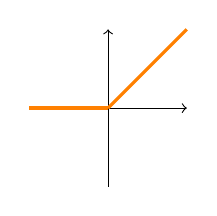
\begin{tikzpicture}
\draw[->] (-1,0) -- (1,0) ;
\draw[->] (0,-1) -- (0,1) ;
\draw[very thick, color=orange]  (0,0) -- (1,1) ;
\draw[very thick, color=orange] (-1,0) -- (0,0)  ;
\end{tikzpicture}

\end{flushleft}

\begin{flushleft}
$\rho(s) = [MAX\{0,s\}]^2$\\
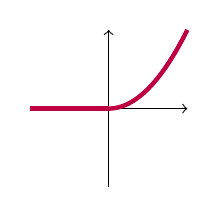
\begin{tikzpicture}
\draw[->] (-1,0) -- (1,0) ;
\draw[->] (0,-1) -- (0,1) ;
\draw[ultra thick, color=purple] (-1,0) -- (0,0)  ;
\draw[ultra thick,purple,domain=0:1,smooth] plot (\x,{(\x)^2}) ;

\end{tikzpicture}

\end{flushleft}
\pagebreak
\item تابع $\psi$
می تواند به صورت های زیر انتخاب شود.
\\

\begin{flushleft}

$\psi (s) = |\psi| $\\
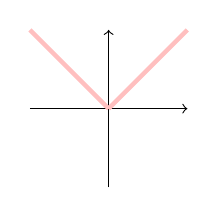
\begin{tikzpicture}

\draw[->] (-1,0) -- (1,0) ;
\draw[->] (0,-1) -- (0,1) ;
\draw[ultra thick, color=pink]  (0,0) -- (1,1)  ;
\draw[ultra thick, color=pink] (-1,1) -- (0,0)  ;

\end{tikzpicture}\\

$\psi(s) = \psi^2 $\\
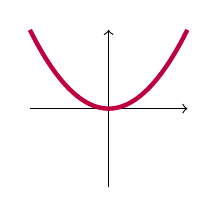
\begin{tikzpicture}

\draw[->] (-1,0) -- (1,0) ;
\draw[->] (0,-1) -- (0,1) ;
\draw[ultra thick,purple,domain=-1:1,smooth] plot (\x,{(\x)^2}) ;

\end{tikzpicture}
\end{flushleft}
\end{itemize}

مساله بهینه سازی 
%\frac{$f(x)=0$}{$g(x)=0$}
\begin{tabular}{ r | c  l }
  $f(x)$ & min\\
$g_i(x)=0$ & s.t\\
 $h_j(x)=0$ & \\
    $x\in \mathbb{R}^n$  &
\end{tabular}
را در نظر می گیریم و متناظر با مساله مقید فوق مساله نامقید زیررا درتعریف می کنیم
\\
\begin{flushleft}


${min} \{f(x)+\underbrace{\mu}_\text{یک عدد حقیق مثبت}\overbrace{ p(x)}^\text{یک تابع جریمه}\}$
\\

$ x\in \mathbb{R}^n$ 

\end{flushleft}

\end{document}
